\subsubsection{Bioacoustic Index Visualization}
For the Bioacoustic index, the value output by the algorithms is an area value under a curve for both the left and right channels where relevant. Thus initially, the best representation of this index would be a stacked area graph, with both the left and right channels included.\\

\begin{center}
	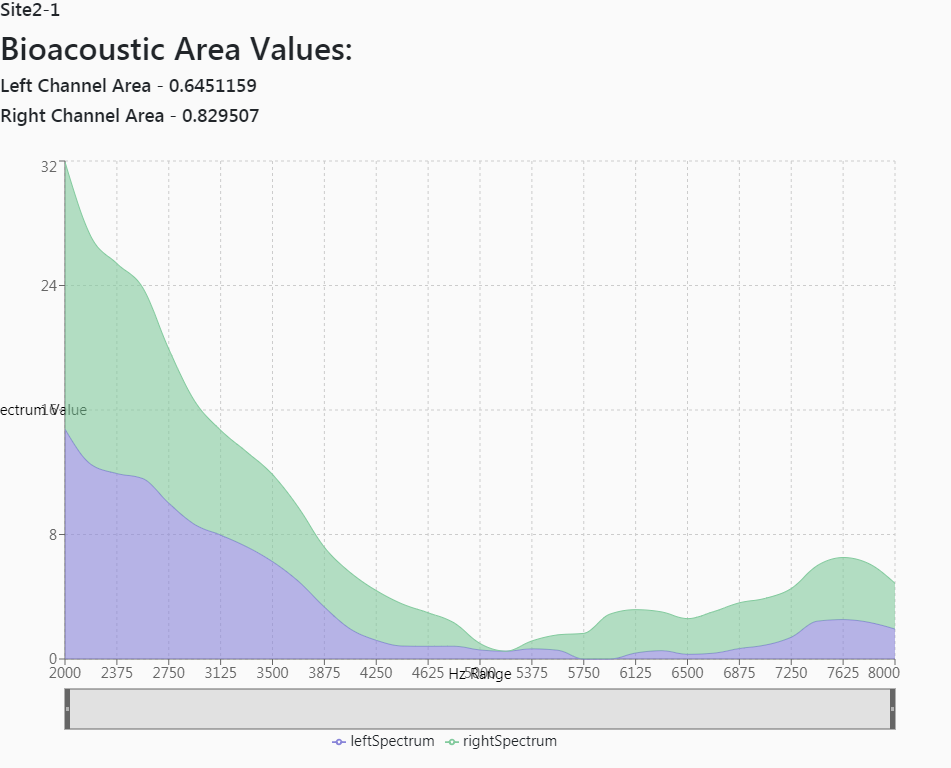
\includegraphics[width=\textwidth]{BAgraph1} \\[12pt]
\end{center}
This graph includes both channels, with a brush included much like in ACI. Because the index calculates a literal area under a curve, an area chart is logically the best representation, and the graphic helps to support this. Again, the user can filter by hertz range using the brush, giving insight into the values in specific ranges. This particular graph is comparing two files in from the same site, but different series. This helps to show the distinct difference in BI values between the two.\\
